\documentclass[xcolor=dvipsnames]{beamer}
\usepackage[utf8]{inputenc}
\usepackage{xcolor}
\usepackage{graphicx}
\usepackage{MnSymbol}
\usepackage{stmaryrd}
\usepackage{colortbl}
\usepackage{caption}
\usepackage{comment}
\usepackage[utf8]{inputenc}
\usepackage{pdfpages}
\usepackage{listings}
\usepackage{color}
\usepackage{booktabs}
\usepackage{soul}
\usepackage[normalem]{ulem}


\usepackage{tcolorbox}
\usepackage{lipsum}


%%%%%%%%%%%%%%%%%%%%%%%%%%%%%%%%%%%%%%%%%%%%%%%%%

\usepackage{pgf}
%\usepackage{etex}
\usepackage{tikz,pgfplots}
\usetikzlibrary{matrix,arrows,decorations.pathmorphing}
\usetikzlibrary{tikzmark}

%\usetheme{Antibes}
\usetheme{AnnArbor}
%\usecolortheme[named=Maroon]{structure}
\usecolortheme{dolphin}
\usefonttheme{professionalfonts}
\useoutertheme{infolines}
\useinnertheme{circles}



\newcommand{\Ep}{\mathbb{E}}
\newcommand{\Real}{\mathcal{R}}
\newcommand{\Rating}{\mathbf{X}}
\newcommand{\Loss}{\mathcal{L}}

%%%%%%%%%%%%%%%%%%%%%%%%%%%%%%%%%%%%%%%%%%%%%%%%%


\title[Non-Compensatory Recommendation]{Non-Compensatory Psychological Models for Recommender Systems}
\author[Chen Lin]{Chen Lin, Xiaolin Shen, Si Chen\inst{1} \\ Muhua Zhu, Yanghua Xiao \inst{2}}
\institute[XMU]{
\inst{1}
Xiamen University \\
\inst{2}
Alibaba Group \\
}
%\logo{\includegraphics[height=0.5cm]{Bilder/TUBerlinLogo.png}}
\date{18-Dec-2018}
\logo{\pgfimage[height=1.2cm]{BigDIA_logo.jpg}}
\titlegraphic{\includegraphics[height=0.8cm]{xmu_logo.jpg} \includegraphics[height=1cm]{Alibaba_logo.jpg}}

\begin{document}

\AtBeginSection[]{
  \begin{frame}
  \vfill
  \centering
  \begin{beamercolorbox}[sep=8pt,center,shadow=true,rounded=true]{title}
    \usebeamerfont{title}\insertsectionhead\par%
  \end{beamercolorbox}
  \vfill
  \end{frame}
}


\begin{frame}
  \titlepage
\end{frame}

\begin{frame}
\frametitle{Outline}
\tableofcontents
\end{frame}



\begin{frame}{Research Question}
    \begin{itemize}
        \item Q1: How do we explain existing recommendation models from a psychological perspective?
        \item Q2: How can we develop explainable and accurate recommendation models that operate differently from existing models?
    \end{itemize}
\end{frame}

\section{Compensatory Models}

\subsection{Background}

\begin{frame}{Rating Models}
        \begin{itemize}
            \item Goal: reconstruct ratings
            \begin{equation}\label{equ:ratingloss}
\min_{\Theta=\{U,V\}} \Loss(\Theta)=\sum_{u,q}(\Rating_{u,q}-\hat\Rating_{u,q})^2 + \lambda_U\|\mathbf{U}\|^2_2+\lambda_V\|\mathbf{V}\|^2_2
\end{equation}
            \item MF: \begin{equation}\label{equ:MF}
 \hat{\mathbf{X}}_{u,q}=\sum_{k=1}^{K} \mathbf{q}_k \mathbf{u}_k
\end{equation}
\item AMF
 \begin{equation}\label{equ:AMF}
\hat{\Rating}_{u,q}=\sum_{k=1}^{K} \mathbf{q}_{k} (\sum_{\mathbf{p} \in R(u)} \mathbf{p}_k/\sqrt{|R(u)|} ),
\end{equation}
\item LLORMA
\begin{equation}\label{equ:LLORMA}
\hat{\Rating}_{u,q} = \sum_{t=1}^{S} \sum_{k=1}^K \mathbf{u}_{t, k} \frac{K((\mathbf{u}_t,\mathbf{i}_t),(\mathbf{u},\mathbf{q}))}{\sum_{s=1}^{S} K((\mathbf{u}_s,\mathbf{i}_s),(\mathbf{u},\mathbf{q}))} \mathbf{q}_{t,k}
\end{equation}

        \end{itemize}
    
\end{frame}

\begin{frame}{Ranking Models}
    \begin{itemize}
        \item Goal: reconstruct pairwise rankings $p\succ_u q$
        \begin{eqnarray}\label{equ:BPRloss}
\min_{\Theta=\{U,V\}}\Loss(\Theta) =& -\sum_{u}\sum_{p,q} I(p\succ_u q) \log Pr(p\succ_u q)\\\nonumber
& + \lambda_U\|\mathbf{U}\|^2_2+\lambda_V\|\mathbf{V}\|^2_2,
\end{eqnarray}
\item Thurstone Model
\begin{equation}\label{equ:BPR}
Pr(p\succ_u q) = \frac{1} {1+\exp[-(\hat{\Rating}_{u,p}-\hat{\Rating}_{u,q})]}
\end{equation}
\item Bradley-Terry Model
\begin{equation}\label{equ:BT}
Pr(p\succ_u q) = \frac{{\hat{\Rating}_{u,p}}}{{\hat{\Rating}_{u,p}}+ {\hat{\Rating}_{u,q}}},
\end{equation}
    \end{itemize}
\end{frame}
\subsection{Decision Process}

\begin{frame}{Compensatory Decision Rule}

\alert{The decision rule is compensatory because a good performance on one aspect compensates for bad performances on other aspects.}
\centering 
    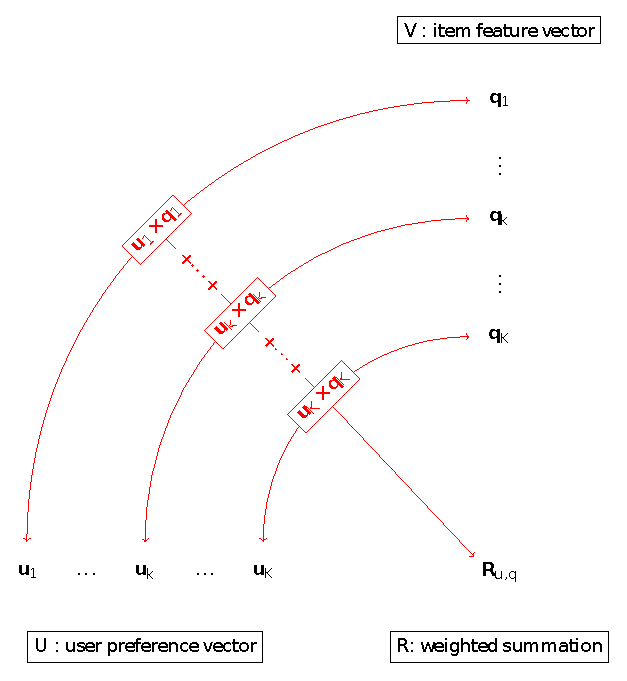
\includegraphics[width=0.4\textwidth]{presentation.eps}



\end{frame}

\begin{frame}{Summary: Related Work}
\centering
    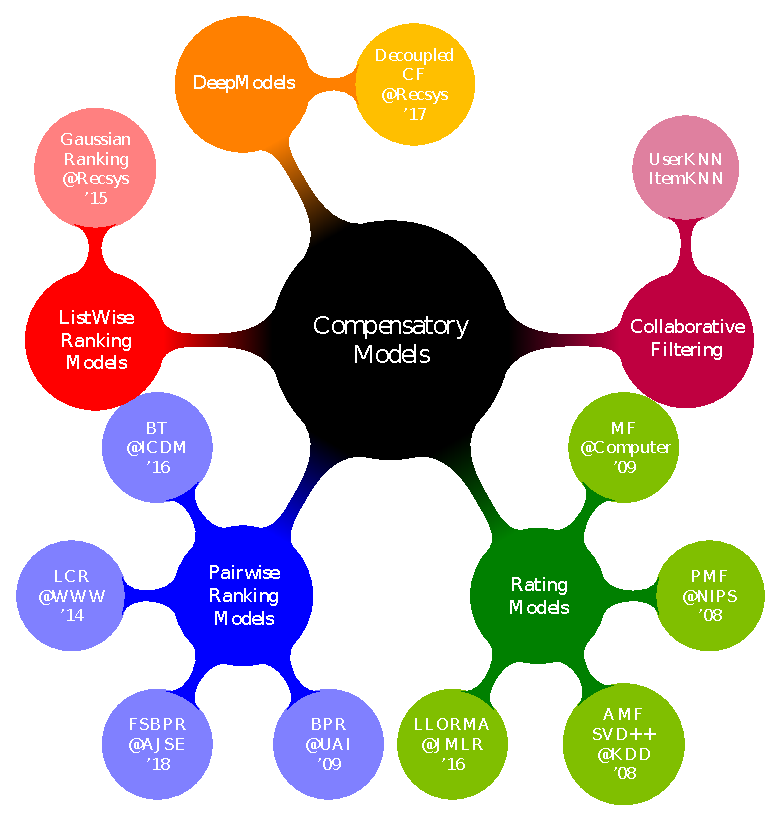
\includegraphics[width=0.6\textwidth]{mindmap.eps}
\end{frame}
\section{Non-Compensatory Models}

\subsection{Motivation}

\begin{frame}{Non-Compensatory Decision Rules}
\begin{itemize}
    \item Lexicographic Rules: order aspects in terms of importance, evaluate items sequentially based on performances  
    \item Conjunctive Rules: items must satisfy a cut-off point on each aspect
    \item Disjunctive Rules: eliminate items that do not satisfy requirement on an important aspect
\end{itemize}
    \begin{table}[htp]
\caption{A cellphone example to illustrate non-compensatory rules.}
\small
\centering
\begin{tabular}{|c|c|c|c|}
\hline
Item & Prominent aspect & \multicolumn{2}{|c|}{Non-prominent aspects}\\\hline
& Battery life &  Price & Memory \\\hline
iPhone SE &  13 hours & 700$\$$ & 64GB  \\\hline
Galaxy S8 & 9 hours& 500$\$$  & 128GB \\\hline
Honor 10 & 24 hours& 589$\$$ & 128GB \\\hline
\end{tabular}
\label{tab:example}
\end{table}
\end{frame}

\begin{frame}{Conceptual Model}
    \begin{block}{Challenge}
    Turn symbolic rules to a data-driven learning framework 
    \end{block}
\centering
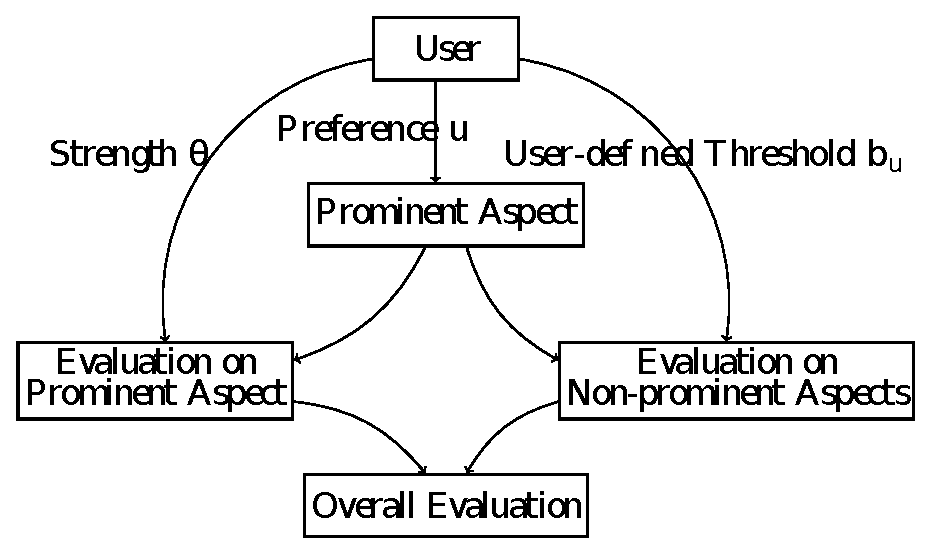
\includegraphics[width=0.7\textwidth]{conceptualmodel.eps}
\end{frame}

\subsection{Rating Models}
\begin{frame}{Non-Compensatory Rating Predictions}
\begin{exampleblock}{Combination of Lexicographic Rules and Conjunctive Rules}
\[
 \hat{\mathbf{X}}_{u,q}=\sum_{k=1}^{K} \tikzmark{s}\frac{\exp \mathbf{u}_k}{\sum_{k'} \exp \mathbf{u}_{k'}} [ \mathbf{q}_k  \exp\theta \tikzmark{a} + \sum_{k'\neq k} (\mathbf{q}_{k'}-\mathbf{b}_{u,k'}) ]\tikzmark{b}
\]

\begin{tikzpicture}[
  remember picture,
  overlay,
  expl/.style={draw=orange,fill=orange!30,rounded corners},
  arrow/.style={red!80!black,ultra thick,->,>=latex}
]
\node<2->[expl] 
  (sex) 
  at (2,-2cm)
  {Choice of prominent aspect};
\node<2->[expl] 
  (aex) 
  at (6,-3cm)
  {Lexicographic rule};
\node<2->[draw=orange,fill=orange!30,rounded corners,text width=3cm] 
  (bex) 
  at (10.5,-1.5cm)
  {Conjunctive rule, cut-off: $b_{u,k'}$};
\draw<2->[arrow]
  (sex) to[out=100,in=180] ([yshift=0.5ex]{pic cs:s});  
\draw<2->[arrow]
  (aex.east) to[out=0,in=-90] ([xshift=0.5ex]{pic cs:a});  
\draw<2->[arrow]
  (bex.north) to[out=90,in=0] ([yshift=0.5ex]{pic cs:b});  
\end{tikzpicture}
\end{exampleblock}
\end{frame}

\begin{frame}{Realization to Rating Models}

         \begin{itemize}
         \item Goal: reconstruct ratings
             \begin{equation}\label{equ:ratingloss}
\min_{\Theta=\{U,V,\theta,b\}} \Loss(\Theta)=\sum_{u,q}(\Rating_{u,q}-\hat\Rating_{u,q})^2 + \lambda_U\|\mathbf{U}\|^2_2+\lambda_V\|\mathbf{V}\|^2_2
\end{equation}
            \item MF-N: 
            \begin{equation}\label{equ:MF-N}
 \hat{\mathbf{X}}_{u,q}=\sum_{k=1}^{K} \frac{\exp \mathbf{u}_k}{\sum_{k'} \exp \mathbf{u}_{k'}} [ \mathbf{q}_k  \exp\theta  + \sum_{k'\neq k} (\mathbf{q}_{k'}-\mathbf{b}_{u,k'}) ]
\end{equation}
\item AMF-N
 \begin{eqnarray}\label{equ:AMF-N}
 \hat{\mathbf{X}}_{u,q}=&\sum_{k=1}^{K} \frac{\exp (\sum_{\mathbf{p} \in R(u)} \mathbf{p}_k )}{\sum_{k'} \exp  (\sum_{p \in R(u)} \mathbf{p}_{k'} ) } \\\nonumber
& [  \mathbf{q}_k \exp\theta + \sum_{k'\neq k} (\mathbf{q}_{k'}-\mathbf{b}_{u,k'}) ].
\end{eqnarray}
\item LLORMA-N
\begin{eqnarray}\label{equ:LLORMA-N}
\hat{\Rating}_{u,q} = & \sum_{t=1}^{S} \sum_k  \frac{\exp \mathbf{u}_k}{\sum_{k'} \exp \mathbf{u}_{k'}}  \frac{K((\mathbf{u}_t,\mathbf{i}_t),(\mathbf{u},\mathbf{q}))}{\sum_{s=1}^{S} K((\mathbf{u}_s,\mathbf{i}_s),(\mathbf{u},\mathbf{q}))} \\\nonumber
& [ \mathbf{q}_{t,k} \exp\theta  + \sum_{k'\neq k} (\mathbf{q}_{t,k'}-\mathbf{b}_{u,k'}) ]
\end{eqnarray}

        \end{itemize}
        
 %     \end{tikzpicture}
\end{frame}


\subsection{Ranking Models}
\begin{frame}{Non-Compensatory Thurstone Model}
\begin{equation}\label{equ:BPR}
Pr(p\succ_u q) = \frac{1} {1+\exp[-(\hat{\Rating}_{u,p}-\hat{\Rating}_{u,q})]}
\end{equation}
\begin{block}{Inference}
\begin{itemize}
\item Goal: reconstruct rankings
             \begin{eqnarray}\label{equ:BPRloss}
\min_{\Theta=\{U,V\}}\Loss(\Theta) =& -\sum_{u}\sum_{p,q} I(p\succ_u q) \log Pr(p\succ_u q)\\\nonumber
& + \lambda_U\|\mathbf{U}\|^2_2+\lambda_V\|\mathbf{V}\|^2_2,
\end{eqnarray}
    \item Stochastic Gradient Descent
    \begin{itemize}
       
    \item $\frac{\partial \Loss}{\partial \Theta}=\frac{\partial \Loss'}{\partial \Theta}+ \lambda_U \mathbf{U} + \lambda_V \mathbf{V}$
    \item $\frac{\partial \Loss'}{\partial \Theta}=  \sum_u \sum_{p\succ_u q} \frac{\partial \Loss'}{\partial \Delta\hat{\Rating}_{u,p,q} } \frac{\partial \Delta\hat{\Rating}_{u,p,q}  }{\partial \Theta}$, where $\Delta\hat{\Rating}_{u,p,q} =\hat{\Rating}_{u,p}-\hat{\Rating}_{u,q}$
    \end{itemize}
\end{itemize}
    \end{block}
\end{frame}

\begin{frame}{Non-Compensatory Bradley Terry Model}
    \begin{exampleblock}{Combination of Lexicographic Rules and Conjunctive Rules}
\[
Pr(p\succ_u q)  =  \sum_{k=1}^{K} \tikzmark{s}\mathbf{u}_k [ {\frac{\mathbf{p}_k}{\mathbf{p}_k+\theta \mathbf{q}_k}}\tikzmark{a} \prod_{k'\neq k}{ \frac{\theta \mathbf{p}_{k'}}{\mathbf{q}_{k'}+\theta \mathbf{p}_{k'}}}]\tikzmark{b}\]

\begin{tikzpicture}[
  remember picture,
  overlay,
  expl/.style={draw=orange,fill=orange!30,rounded corners},
  arrow/.style={red!80!black,ultra thick,->,>=latex}
]
\node<2->[expl] 
  (sex) 
  at (2,-2cm)
  {Choice of prominent aspect};
\node<2->[expl] 
  (aex) 
  at (6,-3cm)
  {Lexicographic rule, $\mathbf{p}_{k} > \theta \mathbf{q}_{k}, \theta>1$};
\node<2->[expl,text width=3cm] 
  (bex) 
  at (10.5,-1.5cm)
  {Conjunctive rule cut-off: $q_{k'}/\theta$};
\draw<2->[arrow]
  (sex) to[out=100,in=180] ([yshift=0.5ex]{pic cs:s});  
\draw<2->[arrow]
  (aex.east) to[out=0,in=-90] ([xshift=0.5ex]{pic cs:a});  
\draw<2->[arrow]
  (bex.north) to[out=90,in=0] ([yshift=0.5ex]{pic cs:b});  
\end{tikzpicture}
\end{exampleblock}
\end{frame}

\begin{frame}{Inference}
\begin{itemize}
    \item Stochastic EM
    \item Sample $k$
    \begin{equation}
 k \sim u_k^{t} \frac{\mathbf{p}_{k}^t} {\mathbf{p}_{k}^t+\theta^t \mathbf{q}_{k}^t} \prod_{k'\neq k}  [\frac{\theta^t \mathbf{p}_{k'}^t} {\mathbf{q}_{k'}^t + \theta^t \mathbf{p}_{k'}^t}].
 \end{equation}
 \item MM-bound
 \begin{eqnarray}
     \Loss \geq & \sum_u \sum_{d\in D(u)} \{\log  u_k  + [ 1- \frac{w_k+\theta l_k}{ w_k^t + \theta^t l_k^t}  + \log \frac{w_{k}} {w_{k}^t+\theta ^t l_{k}^t} ] \\\nonumber 
     & \sum_{k'\neq k}  [ 1- \frac{ l_{k'}+\theta w_{k'}}{ l_{k'}^t+\theta^t w_{k'}^t}  + \log \frac{\theta w_{k'}} {l_{k'}^t+\theta ^t w_{k'}^t} ] \}
 \end{eqnarray}
\end{itemize}
    
\end{frame}
\section{Experimental Analysis}
\subsection{Rating Prediction}

\begin{frame}{Data Sets}
    \begin{table}[htp]
\caption{Statistics of Datasets with ratings}
\small
\centering
\scalebox{0.9}{
\begin{tabular}{|c|c|c|c|c|}
\hline
Dataset & \#users & \#items & \#ratings & \#pairs \\\hline
Movielens &942 &1,650 &80,000 & 1,072,237 \\\hline
Filmtrust &1,235 &2,062 &35,497 &623,516 \\\hline
CiaoDVD &2,665 &14,280 &72,665 &2,478,836 \\\hline
\end{tabular}}
\label{tab:datasets}
\end{table}
\end{frame}

\begin{frame}{Results}
    \begin{table}[htp]
\tiny
\centering
\scalebox{0.9}{
\begin{tabular}{c cc |cc |cc}
\hline
Method & AUC & Imp.& NDCG& Imp.& MRR &Imp.\\\hline
Movielens& & $(\%)$ & & $(\%)$ & & $(\%)$\\\hline
MF&	0.6729 &	&	0.6925 &	&	0.8300 &	\\
MF-N&	0.7108 &	5.62&	0.7166 &	3.48&	0.8633 &	4.01\\
AMF&	0.6901 &	&	0.7107 &	&	0.8747 &	\\
AMF-N &	0.7027 	&1.83&	0.7138 &	0.44&	0.8790 	&0.49\\
LLORMA&	0.7265 &	&	0.8734 &	&	0.7015 &	\\
LLORMA-N&	0.7299 &	0.47&	0.8999 &	3.03&	0.7187 &	2.45\\\hline
Filmtrust& & $(\%)$ & & $(\%)$ & & $(\%)$\\\hline
MF&	0.6507 &	&	0.5229 &	&	0.7011 &	\\
MF-N&	0.6710 &	3.12&	0.5241 &	0.23&	0.7071 &	0.86\\
AMF&	0.5971 &	&	0.5137 &	&	0.7411 &	\\
AMF-N&	0.6133 &	2.71&	0.5253 &	2.25&	0.7619 &	2.80\\
LLORMA&	0.6240 &	&	0.8596 &	&	0.7857 &	\\
LLORMA-N&	0.6345 &	1.68&	0.8684 &	1.02&	0.8068 &	2.69\\\hline
CiaoDVD& & $(\%)$ & & $(\%)$ & & $(\%)$\\\hline
MF&	0.7431 &	&	0.7949 &	&	0.8910 &	\\
MF-N&	0.7903 &	6.34&	0.8127 &	2.25&	0.9154 &	2.74\\
AMF&	0.6489 &	&	0.6612 &	&	0.8741 &	\\
AMF-N&	0.6993 &	7.77&	0.6878 &	4.02&	0.8967 &	2.58\\
LLORMA&	0.6752 &	&	0.7827 &	&	0.8267 &	\\
LLORMA-N&	0.6845 &	1.38&	0.7984 &	2.00&	0.8384 &	1.42\\
\hline
\end{tabular}}
\label{tab:ratingresult}
\end{table}

\end{frame}



\subsection{Ranking for Explicit Feedbacks}

\begin{frame}{Results}
    \begin{table}[htp]
\tiny
\centering
\scalebox{0.9}{
\begin{tabular}{c cc|cc|cc}
\hline
 Method & AUC & Imp.& NDCG& Imp.& MRR &Imp. \\\hline
Movielens& & $(\%)$ & & $(\%)$ & & $(\%)$\\\hline
BT&0.6453 & & 0.5329 & & 0.8227 & \\
BT-N& 0.8511 & 31.89& 0.5795 & 8.74& 0.9256 & 12.51\\
BPR	&0.7976	&&	0.5674	&&	0.8988	&\\
BPR-N	&0.8361	&4.82&	0.5761&	1.53&0.9180	&2.14\\
FSBPR	&0.5048 	&&	0.5011 	&&	0.7524 	&\\
FSBPR-N&	0.8272 &63.86&	0.5740 &	14.56&	0.9136 &	21.42\\
LCR&	0.7191&&		0.8555&&		0.9461	&\\
LCR-N&	0.7360	&2.35&	0.8605&	0.58&	0.9515&	0.57\\
\hline
FIlmtrust& & $(\%)$ & & $(\%)$ & & $(\%)$\\\hline
BT& 0.5405 & & 0.5092 & & 0.7702 & \\
BT-N & 0.6969 & 28.94& 0.5446 & 6.95& 0.8485 & 10.15\\
BPR&	0.6412	&&	0.5319	&&	0.8206&\\	
BPR-N	&0.6729	&4.94&	0.5391	&1.35&	0.8364&	1.93\\
FSBPR	&0.4857 	&&	0.4968 &&		0.7428 	&\\
FSBPR-N	&0.6717 &	38.29&	0.5388 &	8.47&	0.8358 &	12.52\\
LCR	&0.5977&&		0.9034	&&	0.7511	&\\
LCR-N&	0.6144&	2.79&	0.9063	&0.32&	0.7635	&1.65\\
\hline
CiaoDVD& & $(\%)$ & & $(\%)$ & & $(\%)$\\\hline
BT& 0.6063 & & 0.5240 & & 0.8031 & \\
BT-N& 0.9334 & 53.95& 0.5981 & 14.1& 0.9666 & 20.36\\
BPR	&0.6344	&&	0.5304&&		0.8172	&\\
BPR-N	&0.8987	&41.66&0.5902&	11.28&	0.9493&	16.17\\
FSBPR	&0.7537 	&&	0.5574 	&&	0.8769 	&\\
FSBPR-N&	0.8992 &	19.30&	0.5903 &	5.91&	0.9496 &	8.30\\
LCR&	0.6260	&&	0.9408	&&	0.7889	&\\
LCR-N	&0.6349&	1.42&	0.9451&	0.46&	0.7988&	1.25\\
\hline
\end{tabular}}
\label{tab:rankingresult}
\end{table}
\end{frame}

\subsection{Ranking for Implicit Feedbacks}

\begin{frame}{Data Sets}
    \begin{table}[htp]
\caption{Statistics of Datasets with graded implicit feedback}
\small
\centering
\scalebox{0.9}{
\begin{tabular}{|c|c|c|c|c|}
\hline
Dataset & \#users & \#items & \#pairs & \#sessions \\\hline
Tmall-single &33,815 &176,231 &5,682,833 &364,844 \\\hline
Tmall-hybrid &62,101 &198,344 &6,072,061 &475,503 \\\hline
Yoochoose &341,396 &30,852 &3,044,572 &341,396 \\\hline
\end{tabular}
}
\label{tab:idata}
\end{table}%
\end{frame}

\begin{frame}{Results}
    \begin{table}[ht]
\tiny
\centering
\scalebox{0.9}{
\begin{tabular}{c cc |cc |cc|cc|cc}
\hline
Method	& AUC	& Imp.($\%$)&	NDCG&	Imp.($\%$)&	MRR	&Imp.($\%$) &	MAP&	Imp.($\%$)&	Prec	&Imp.($\%$)\\\hline
Tmall-single\\\hline
BT	&0.5304 	&	&0.2804 	&	&0.4870 	&	&0.4327 	&	&0.2778 &\\
BT-N	&0.5400 	&1.82	&0.2840 	&1.28	&0.4948 	&1.61	&0.4386 	&1.34	&0.2801 & 0.84\\
BPR&	0.5181	&&	0.2794	&&	0.4854	&&	0.4297	&&	0.2767&\\	
BPR-N	&0.5349&	3.24&	0.2848	&1.92&	0.4960	&2.18&	0.4401&	2.41&	0.2806	&1.41\\
FSBPR	&0.5265 	&&	0.2824 	&&	0.4913 	&&	0.4350 	&&	0.2794 	&\\
FSBPR-N	&0.5389& 	2.35&	0.2863 	&1.39&	0.4988 &	1.53&	0.4432 &	1.90&	0.2818 &	0.87\\
LCR&	0.5200 	&&	0.8190 	&&	0.4277 	&&	0.3568 	&&	0.2534 	&\\
LCR-N&	0.5290 &	1.73&	0.8213 &	0.28&	0.4360 	&1.94&	0.3648 	&2.24&	0.2586 &	2.05\\
\hline
Tmall-hybrid\\\hline
BT	&0.5867 	&	&0.3015 	&	&0.5373 	&	&0.4929 	&	&0.2904 & \\
BT-N	&0.6568 	&11.94	&0.3279 	&8.75	&0.5990 	&11.48	&0.5527 	&12.13	&0.3036 &4.53 \\
BPR	&0.6183&	&	0.3183&&		0.5792	&&	0.5318&&		0.2973&\\	
BPR-N	&0.6460	&4.48&	0.3276&	2.92&0.5990	&3.41&	0.5524&	3.87&	0.3030	&1.94\\
FSBPR	&0.6334 	&&	0.3246 	&&	0.5916 &&		0.5442 	&&	0.3026 	&\\
FSBPR-N&	0.6544 &	3.31&	0.3309 &	1.94&	0.6062 &	2.48&	0.5603 &	2.95&	0.3047 &	0.69\\
LCR	&0.5398 	&&	0.6644 	&&	0.4519 	&&	0.3745 	&&	0.2597 	&\\
LCR-N&	0.5649 &	4.65&	0.6790 &	2.20&	0.4809 &	6.42&	0.3988 &	6.49&	0.2720 &	4.74\\
\hline
Yoochoose\\\hline
BT	&0.6027 	&	&0.4734 	&	&0.7151 	&	&0.6361 	&	&0.4560 & \\
BT-N	&0.7000 	&16.15	&0.5160 	&8.99	&0.7869 	&10.04	&0.7084 	&11.37	&0.4785  &4.92\\
BPR&	0.6700	&&	0.5065	&&	0.7713&&		0.6895	&&	0.4737&\\	
BPR-N	&0.6920	&3.28&	0.5131	&1.31&	0.7812&	1.29&	0.7027	&1.91&	0.4771	&0.74\\
FSBPR	&0.3272 	&&	0.3658 	&&	0.5062 	&&	0.4599 	&&	0.4006 	&\\
FSBPR-N	&0.6198 &	89.45&	0.4822 &	31.83&	0.7169& 	41.62&	0.6448 &	40.22&	0.4650 &	16.08\\
LCR	&0.5842 	&&	0.9725 	&&	0.8009 &&		0.7934 	&&	0.7677 	&\\
LCR-N&	0.6315 &	8.10&	0.9754 &	0.30&	0.8231 &	2.77&	0.8161 &	2.86&	0.7881 &	2.66	\\
\hline
\end{tabular}}
\label{tab:gradedresult}
\end{table}
\end{frame}
\begin{frame}{Parameters}
    
\begin{table}[htp]
\caption{AUC improvements with $\mathbf{b}$ activated, scale of parameters $\mathbf{b}_{u,k}$ and $\theta$.}
\small
\centering
\scalebox{0.9}{
\begin{tabular}{c|c|c |c}
\hline
Dataset   &Imp.($\%$)& $\sigma(\mathbf{b}_{u})$& $\theta$ \\\hline
Movielens & 5.37 & $0.0095\pm0.0024$ & $0.608\pm 0.105$  \\
FilmTrust & 2.21 & $0.0095\pm0.0023$ & $0.667\pm 0.016$\\
CiaoDVD & 28.97 & $0.0093\pm0.0022$  &$0.773\pm 0.051$\\\hline
\end{tabular}
}
\label{tab:parameters}
\end{table}
\end{frame}
\begin{frame}{Summary}
        \begin{itemize}
        \item Q1: How do we explain existing recommendation models from a psychological perspective?
        \item \alert{A1: A large body of existing recommendation models are based on compensatory decision rules.}
        \item Q2: How can we develop explainable and accurate recommendation models that operate differently from existing models?
          \item \alert{A2: Applying non-Compensatory rules universally improve recommendation performances.}
    \end{itemize}
\end{frame}
\begin{frame}{Paper and Codes}
    \begin{itemize}
        \item Paper: Chen Lin et.al. Non-Compensatory Psychological Models for Recommender Systems. To appear in AAAI 2019
        \item Codes are available at https://github.com/XMUDM/Non-Compensatory
    \end{itemize}
\end{frame}

%%%%%%%%%%%%%%%%%%%%%%%%%%%%%%%%%%%%%%%%%%%%%%%%%%%
\end{document}
